\documentclass{IEEEtran}
\usepackage{booktabs}
\usepackage{graphicx}
\usepackage{fancyhdr} % ����ҳüҳ��
\usepackage{framed}
\pagestyle{fancy}
\lhead{}
\chead{}
\rhead{}
\lfoot{}
\cfoot{}
\rfoot{\thepage}
\title{Lab 2 Amplifiers}
\author{Group 8: Muhan Li \and Man Sun \and Mingxiao An \\ EE233 Circuit Theory}
\IEEEaftertitletext{\centering \fontsize{11}{11}\textsc{Department of Electrical Engineering, University of Washington, Seattle, WA, 98195}}

\begin{document}
	\maketitle
	\renewcommand{\headrulewidth}{0pt} %��Ϊ0pt����ȥ��ҳü����ĺ���
	\renewcommand{\footrulewidth}{0pt} %��Ϊ0pt����ȥ��ҳ������ĺ��� 0.4pt	
	\begin{abstract}
		this lab report is about the procedure, measurements, and analysis of using an operational amplifier as a voltage follower or summing amplifier. The experiment verified some parameters of op-amp LM348 and a simple audio mixer was finally built using the op-amp.
	\end{abstract}
	\section{Introduction}
	In this lab, we learned how to read and obtain data from integrated circuit component specification sheets through LM348N datasheet, how to do SPICE simulation through Multisim, and the characteristic of operational amplifiers through measuring and analyzing them. \newline
\phantom{ } The characteristic was tested in two sections. In the first section, we experimented the op-amp's characteristic as a voltage follower and compared the testing result with those parameters on the spec. In the second section, we tested the summing amplifier circuit, which is essential for mixing signal channels. We used a speaker and an oscilloscope to display the mixing result, and found out the function of each potentiometer.
	\section{Lab Procedure}
	\textbf{New elements in this lab} \newline
\phantom{ } Since most of the basic elements have been discussed in the report of Lab 1, we will not discuss these elements again. We are going to discuss about the new elements we used in this lab. The two basic elements are 100$ \si{\kilo\Omega} $ resistors and 22$\si{\pico\farad}$ capacitor. The resistor are not like the one we discussed before, we will need to use a potentiometer with a maximum resistance of 100$ \si{\kilo\Omega} $ instead. We can change the resistance of a potentiometer rotating the knob (also remember to connect the middle pin to the circuit). The capacitor is almost same as the one we used to use, but with a different format of label. Also we will need to use Audio Jack, which contains three kinds of wires. The red wire is the high output source and the thick black one should be connected to the ground in the circuit. The other one can be left alone. We also used the op-amp LM348 in this lab. It is an IC-chip with 14 pins. the middle pin of the two sides is respectively $ \mathrm{V_{CC}} $ and $ \mathrm{V_EE} $. It contains 4 groups of pins. In each group, the pins at the ends is the output pin, the ones near the end is $ \mathrm{V_-} $ and the left one is $ \mathrm{V_+} $. The last new element we used is the speaker. It is like a audio player with two input terminals, $ \mathrm{V_+} $ and  $ \mathrm{V_-} $.

	\section{Experimental Procedure and Analysis}
	\subsection{Voltage Follower}
	\hfill \newline
\phantom{ } We first built the circuit on our experimental board according to the circuit in figure[\ref{fig:1.1}].\\
\begin{figure}[!htbp]
	\centering %����
	\begin{framed}
		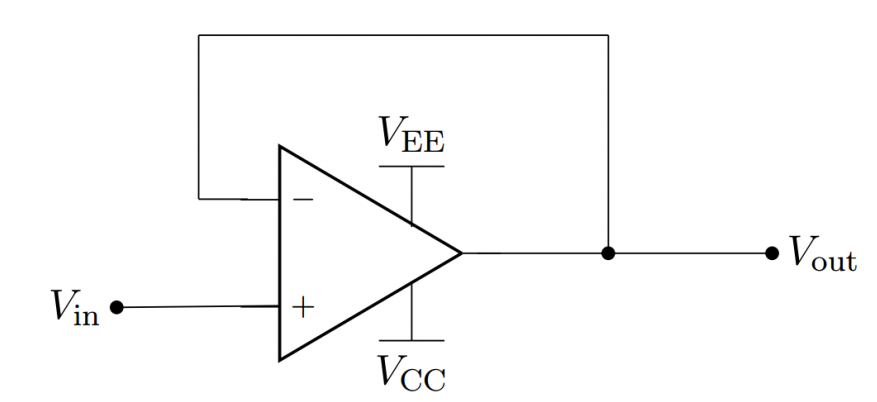
\includegraphics[width=\linewidth]{images/1_1.PNG} %���ȣ��ļ���ַ
		\caption{Voltage follower schematic} %����
		\label{fig:1.1} %��ǣ�����ʱ�ã�
	\end{framed}
	
\end{figure}

\phantom{ } Because our lab equipment can only provide DC source ranging from 0 to 30$ \si{\volt} $, and the op-amp needs a DC source of 12$ \si{\volt} $ and -12$ \si{\volt} $ to work, we will need to make two 12$ \si{\volt} $ DC sources and connect them in a serial. By setting the connecting point between them as the ground, we can get a pair of DC source that meets the requirement. Our on-board connecting schematic is shown in figure[\ref{fig:1.2}].\\
\begin{figure}[!htbp]
	\centering %����
	\begin{framed}
		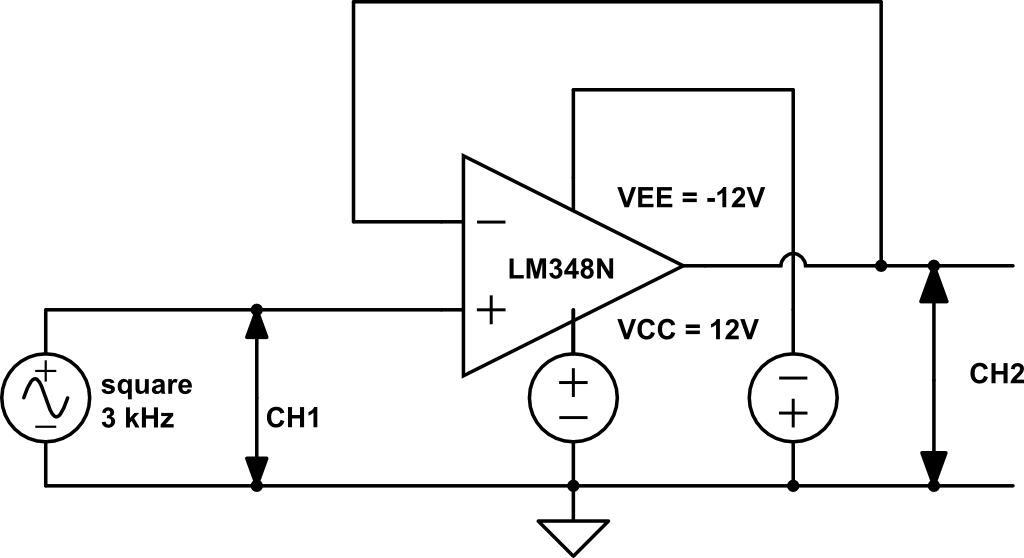
\includegraphics[width=\linewidth]{images/cir1.PNG} %���ȣ��ļ���ַ
		\caption{ Voltage follower schematic} %����
		\label{fig:1.2} %��ǣ�����ʱ�ã�
	\end{framed}
\end{figure}

\textbf{Analyze \#1:} \newline
\phantom{ } Then we set the function generator correctly and get the result, which is shown in figure[3].\\
%\begin{figure}[!htbp]
%	\centering %����
%	\begin{framed}
%		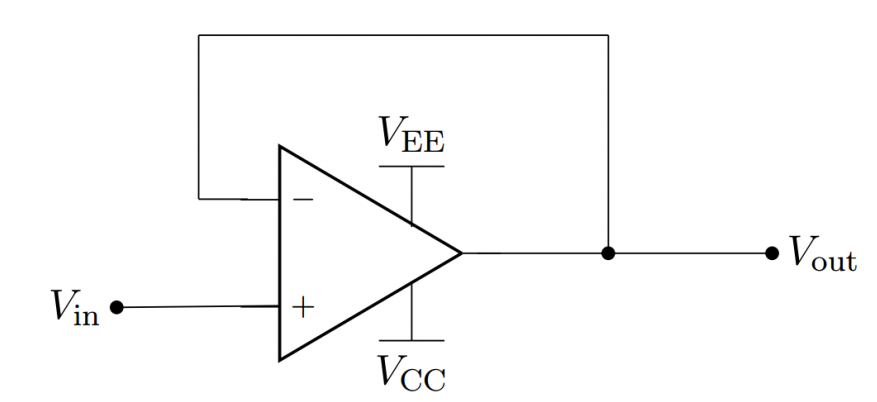
\includegraphics[width=\linewidth]{images/1_1.PNG} %���ȣ��ļ���ַ
%		\caption{ Voltage follower schematic} %����
%	\end{framed}
%	\label{fig:1.1} %��ǣ�����ʱ�ã�
%\end{figure}

\phantom{ } We used the cursor and measured the time needed for the output(CH2) to reach steady state after a drastic change in the input(CH1), which was 21.20$ \mu\si{\second} $. The slew rate is then:\\
\begin{equation}
	\mathrm{SlewRate} = \frac{\Delta \mathrm{V}}{\Delta t} = \frac{20.4\si{V}}{21.20\mu\si{s}} = 0.962\si{V/\mu s}
\end{equation}

\phantom{ } While in the data sheet, the slew rate is 0.5$ \si{V/\mu s} $. But in data sheet, the given slew rate is under the condition of $ \mathrm{V_s} = \pm15\si{V} $. In our experiment,  $ \mathrm{V_s} = \pm12\si{V} $, that is one of the reasons of the difference between these two slew rates.%TODO ��û�����ô˵

\textbf{Analyze \#2:} \newline
\phantom{ } We set the input signal to a sine wave with an amplitude of 3$ \si{\volt} $
 and a frequency of 1$ \si{k\hertz} $. We observed that the follower's output signal followed the input signal perfectly. Then we gradually added the frequency of the input sine wave, and we observed some angels and straight lines in the output signal, which meant the output signal was distorted. We recorded the frequency, %3 analysis
	\subsection{Summing Amplifier}
	\hfill \newline
\phantom{ } Then we built the summing aplifier circuit according to the figure below. We kept the power supply at $ \mathrm{V_s} = \pm12\si{V} $, and set the function generator to provide ${v_1}(t)=cos(2000\pi t)\si{V}$, ${v_2}(t)={v_3}(t)=0$. All resistors were set to $100\si{k\Omega}$ and the capacitor $C=22\si{pF}$.
\begin{figure}[!htbp]
	\centering 
	\begin{framed}
		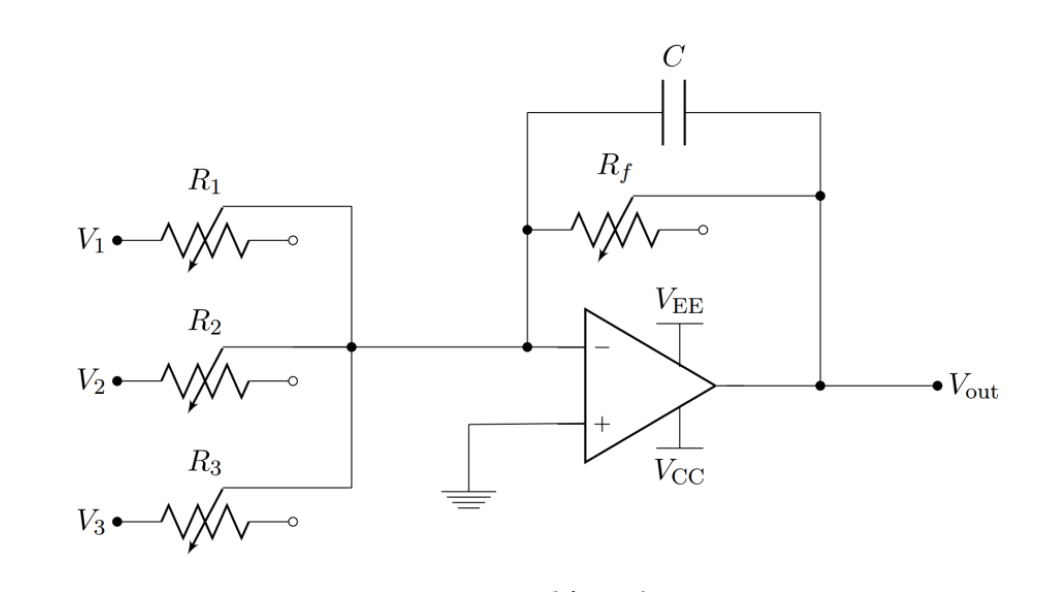
\includegraphics[width=\linewidth]{images/summing_amp.PNG} 
		\caption{Summing amplifier with potentiometers}
		\label{fig:samp} 
	\end{framed}
\end{figure} 

\phantom{ } We swept the frequency of $\mathrm{V_1}$ from 10$\si{\hertz}$ to 1$\si{M\hertz}$, kept the input amplitude same and recorded the amplitude of output signals. The data collected is showed in Table[\ref{tab:caf}], and we got a plotted figure Figure[\ref{fig:afreq}] of the output voltage in terms of frequency.

\begin{table}[!htbp]
	\centering
	\caption{Amplitudes under different frequencies}
	\begin{tabular}{lccllcc}
		\toprule
		No&freq($\si{\hertz}$)&Amp($\si{\volt}$)&&No&freq($\si{\hertz}$)  &Amp($\si{\volt}$)\\
		\midrule
		1	&10		&1.94	&&9 &$5*10^3$&2.02\\
		2	&20		&1.94	&&10&$1*10^4$&2\\
		3	&50		&1.94	&&11&$2*10^4$&1.92\\
		4	&100	&1.94	&&12&$5*10^4$&1.55\\
		5	&200	&1.92	&&13&$1*10^5$&1.05\\
		6	&500	&1.96	&&14&$2*10^5$&0.604\\
		7	&1000	&1.96	&&15&$5*10^5$&0.28\\
		8	&2000	&1.98	&&16&$1*10^6$&0.152\\
		\bottomrule
	\end{tabular}
	\label{tab:caf}
\end{table}

\begin{figure}[!htbp]
	\centering 
	\begin{framed}
		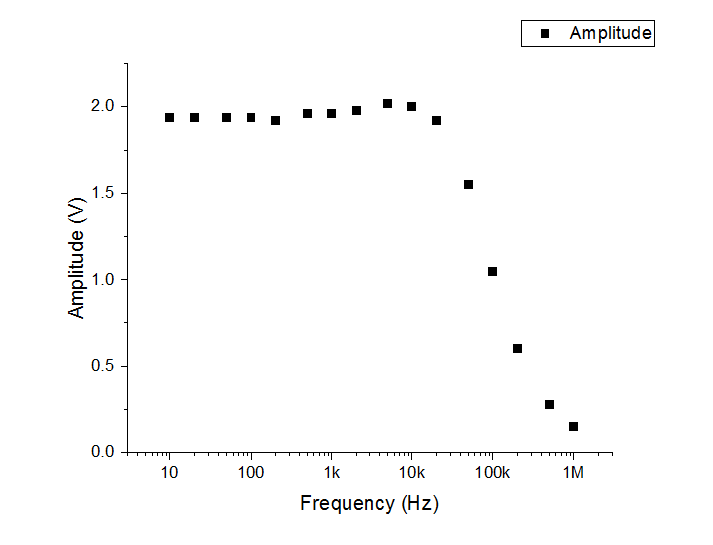
\includegraphics[width=\linewidth]{images/amp_freq.PNG} 
		\caption{Amplitudes under different frequencies}
		\label{fig:afreq} 
	\end{framed}
\end{figure} 

\textbf{Analyze \#4:} \newline
\phantom{ } Comparing our result to Figure[\ref{fig:pre8}] and Figure[\ref{fig:pre11}], which was plotted in Prelab\#8 and \#11, 
\begin{figure}[!htbp]
	\centering 
	\begin{framed}
		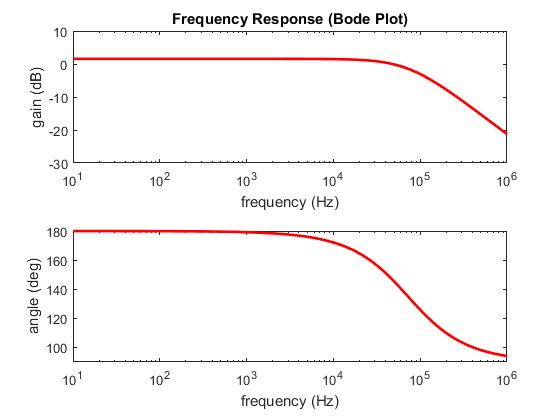
\includegraphics[width=\linewidth]{prelab/images/9_1.PNG} 
		\caption{Magnitude and phase of the output signal}
		\label{fig:pre8} 
	\end{framed}
\end{figure} 
\begin{figure}[!htbp]
	\centering 
	\begin{framed}
		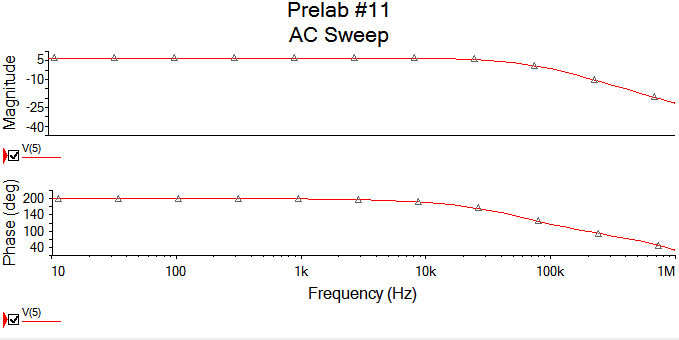
\includegraphics[width=\linewidth]{prelab/images/11_1.PNG} 
		\caption{Magnitude and phase of the output signal}
		\label{fig:pre11} 
	\end{framed}
\end{figure}
\phantom{ } As we can see, our records are in a similar shape with the theoretical result-relatively flat at high frequency, and starts falling around the frequency of 10$ \si{k\hertz} $. The reason for the three graphs falling in different slope is that the y-axis is in different scales and values.\\

\textbf{Analyze \#6:} \newline
\phantom{ } When we adjusted the four potentiometers separately, we found that $ \mathrm{R_f} $ controls the whole volume while other three potentiometers controls the volume of each track respectively. The overall volume will decrease when the potentiometer's resistance decreases. Other three potentiometers controls the volume of the sources that they respectively connected to. The volume of the source that goes through one of these three potentiometers will fall when the nearest potentiometer's resistance falls. % 3 analysis
	\section{Conclusions}
		\hfill \newline
\phantom{ } After finishing all the measurements and analysis, we successfully built the simple audio mixer, and we could adjust the potentiometers to control the volume of each track. We have also discussed why there are a few differences between measured values and values on the spec. The difference structure of the circuit and type of the op-amp are potential reasons.\\

\begin{table}[!htbp]
	\caption{Team Roles}
	\renewcommand\arraystretch{1.5}\centering
	\begin{tabular}{l|c}
		\hline
		\hline
		Activity					&	Student Name 	\\
		\hline
		Prelab/Circuit Analysis		& 	Muhan Li		\\
		\hline
		Prelab/Simulations			&	Mingxiao An		\\
		\hline
		Prelab/answer questions		&	Man Sun			\\
		\hline
		Circuit construction		&	Mingxiao An		\\
		\hline
		Data collection				& Muhan Li, Man Sun	\\
		\hline
		Data analysis				& Muhan Li, Man Sun \\
		\hline
		Lab report writing			& Mingxiao An, Muhan Li, Man Sun \\
		\hline
		\hline
	\end{tabular}\\
\end{table}
	\section{Appendix}
		\input{appendix}
	
\end{document}
